\chapter{The Application}
To achieve the goal presented in section ..., we need to build a scalable program architecture.
To this end, we sketched our idea for the program architecture in the diagram shown in figure \ref{fig:...}.

% Insert figure here

The primary responsibility of the application is to act as a hub for a professor to create a syllabus related to specific programming courses.
The professor must be able to create exercises and specify the expected output required to solve the given exercise.

Students can then enroll in the courses created by the professor, giving them access to the syllabus.
Once enrolled, students are able to view and attempt to solve the exercises contained within the syllabus.

The goal is then to give the professor an overview of how well each student performed.
This is facilitated through a board, accessible only to the professor, which shows which exercises were solved, which exercises were not solved, and different statistics such as how much time was spent on each exercise.

\section{Architecture}
To accomodate a platform that supports the issues described in Section xxxx we have chosen a client-server architecture. 
In this architecture communication betwen the client and server is implemented using the HTTP protocol. 
The front-end component is responsible for the UI for the platform and must provide the users with described as use-cases.
The back-end of the system supports the heavy lifting for the front end system, utilizing computer power of a server rather than the client's browser. 
The platform must first and foremost support usage from many users at the same time. 
Thus the scalability of the system must be thought into its architecture. 
In this section we will describe the evolution of the platform in terms of its architecture.
After each component has been implemented, its scalability has been tested (see Section xxxx).
Based on the results of the scalability tests, the component have either been improved further or tested again, or new functionality for the system implemented. 
Along with each component, a usecase supporting the use of the component has been implemented on the UI if necessary. 


Figure xxx shows the planned architecture of the platform. 

%Describe the following:
%1. The system must be able to provide a suitable UI for the user, but should not use their computer for anything else 
%2. The system must be able to provide some way to execute haskell code and assert whether or not the code is correct. 
%3. .... therefore we choose to split the system into multiple subsystem, each being responsible for providing different functionalities to the full system and can run independently of one another. 
%4. .... by doing this we gain.....

% Why do we choose the front end we do --- why do we have the 'front end backend?' --- Is the front end system only on the client? No? Why not?

\subsection{Back-end system}
\subsubsection{Code runner}
Our system needs to be able to compile and run haskell code on back-end and verify whether this code is syntactically correct or not.
To accomodate this, a code runner module has been implement in a layered architecture (~\cite{roede_aalborg}).
For this type of architecture each component can depend only on components on a lower or same level, thus if component A is on a lower level than component B, component A cannot use component B.
The component is implemented as a HTTP server as seen on Figure \ref{fig:code_runner}.
Whenever the server recieves a HTTP request, a service request is sent to a \textit{code runner} service that in turn writes the content recieved to a Haskell file and invokes the GHC compiler.
If the compilation of the haskell file fails, the code runner will send the GHC compiler's compilation error as response to the service user.
If the file compiles successfully the code runner will then run the executable file and fetch the produced output of the program.
This output is then sent to the service user.
Finally, the response from the code runner, whether successful or not, is redirected back to the client, providing them with information about the compilation and execution of the program.
\begin{figure}
    \centering
    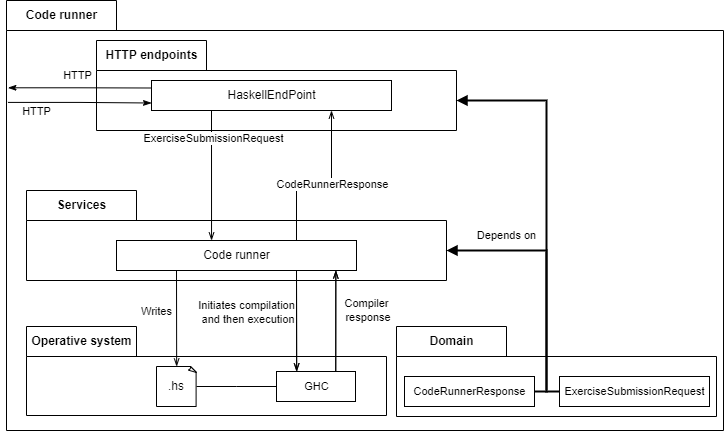
\includegraphics[width=\textwidth,height=\textheight,keepaspectratio]{sections/Chapter 2/pics/P7 arch-Backend - HS compiler.drawio.png}
    \caption[]{The layered architecture of the code runner component for the back end system.}
    \label{fig:code_runner}
\end{figure}

The component's scalability have been measure in Section XXXX. As this result is not satisfactory, further measures to ensure accessibility of the system have been considered. 
First, a queue system for the requests recieved by the component has been implemented. 
Whenever a request hasa been processed by the component and a response sent to the client, the next request in the queue is processed. 
This scalability measure ensures that even if the component is engaged in the processing of many requests, a request will eventually be processed.

\subsection{Front-end system}

\subsubsection{UI}

\subsubsection{UI business layer}